\chapter{Climate Models}\textit{Lecture111}
We will use the shallow water equation, but in order to have a realistic case, we need to put it on the sphere. We start from the usual equation, for convenience we introduce the geopotential $\Phi=gH$:
\begin{align}
    \frac{\partial u}{\partial t}=-u\frac{\partial u}{\partial x}-v\frac{\partial u}{\partial y}+fv-\frac{\partial \Phi}{\partial x}\\
    \frac{\partial v}{\partial t}=-u\frac{\partial v}{\partial x}-v\frac{\partial v}{\partial y}-fu-\frac{\partial \Phi}{\partial y}\\
    \frac{\partial \Phi}{\partial t}=-\frac{\partial u\Phi}{\partial x}-\frac{\partial v\Phi}{\partial y}
\end{align}
Let's use $U=u\cos\phi$, $V=v\cos\phi$, $\vec{V}=\hat{i}U+\hat{j}V$. Until now all the methods we have introduced are designed to give us instruments to simulate and march in the future the atmosphere and the oceans and, probably, much more. What is the difference between all these applications ? 
\begin{enumerate}
    \item Forecasts: The target is the instantaneous state of the system (atmosphere/oceans …) We start at a specific moment that we try to specify as accurately as we can and we want desperately to stay close to the state of the system for as long as we can. 
    \item Climate: The target is the statistics of the system. We want to reproduce its statistical distributions and the initial condition may not be so important, in fact we could start at rest. 
\end{enumerate}
\paragraph{Forcing} Which factors drive the evolution in both cases ?
\begin{enumerate}
    \item Forecasts: The internal dynamics of the atmosphere/ocean is the dominant factor as the initial condition is modified and carried in the future by the processes that we have seen. Conservation properties becomes progressively more important as the range of the forecasts becomes longer. 
    \item Climate: The statistics is influenced by the external forcing and the structure (composition) of the atmosphere and the ocean. For a given external forcing a certain statistics (hopefully only one) will develop in equilibrium with the forcing and a given composition. Conservation properties are important.
\end{enumerate}
\subsection{A climate model}
The radiation wavefront is essentially flat
when it reaches the Earth orbit, therefore it
distributes its energy unequally on the
planet surface.
\begin{equation}\label{e.radiation}
    4\pi R^2F_S=S\pi R^2(1-a)
\end{equation}
The planetary albedo $a$ is about $0.3$, and
the solar constant conventional value is $1361$ W/m$^2$.
\begin{figure}[h!]
    \centering
    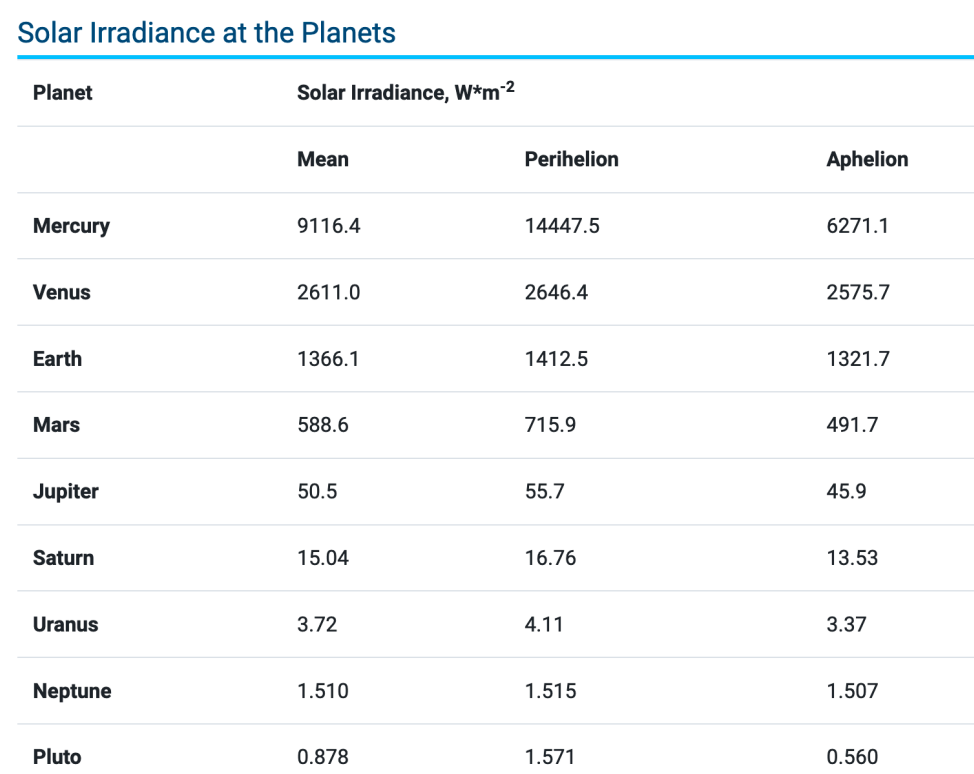
\includegraphics[width=0.5\linewidth]{uploads/Screenshot 2024-11-19 154224.png}
    \caption{Solar Irradiance at the Planets}
    \label{fig:enter-label}
\end{figure}
then
\begin{align*}
    F_S=\frac{S(1-a)}{4}\\
    \sigma T^4= \frac{S(1-a)}{4} \,\,\text{S-B Law} \\
    T=\left(\frac{S(1-a)}{4\sigma}\right)^{1/4}
\end{align*}
with $S=1361$, $a=0.3$ and $\sigma=5.67 \, \, 10^{-8}$, turns out that $T_S=254\text{K}=-18°\text{C}$. This is not the surface temperature that we at the surface, it is considerably colder.However satellite observations are giving us the observed long wave outgoing radiative flux
from the planet outside the atmosphere. In fact it is so detailed that we have seen this flux geographically distributed over the all surface. Its global average is $226\, \, \text{W/m}^2$ from ERA5. With the satellite observations, we can came up with an equation with the observed long wave outgoing radiative flux geographically distributed all over the surface. $OLR_{mean}$ stands for Outgoing Longwave Radiation.
We can use that flux to find the corresponding temperature:
$$\sigma T^4=OLR_{mean}\Longrightarrow T=\left(\frac{OLR}{\sigma}\right)^{1/4}$$
with $OLR=226$ and $\sigma=5.67 \,\, 10^{-8}$
hence, $T_S=251 \text{K}=-21°\text{C}$. This is still not the temperature at the surface, whose global, long term
mean is about $288$ K or $15°$ C, it is though what the satellite sees: it's the level at which emission reaches the out space. There is something that is making the surface opaque, hence the satellite doesn't see the surface but a layer on a higher level (remember that $T$ decreases as the height increases). 
Maybe the earth surface is not really a black body and not all the
radiation reaches outer space, introduce a factor $\tau$, the transmissivity:
$$\tau\sigma T^4=OLR_{mean}$$
and calibrate $\tau$ with the observed surface temperature. 
\begin{equation}\label{eq.tau}
    \tau=\left(\frac{OLR}{\sigma T_S^4}\right)\approx 0.58
\end{equation}
so the observed surface temperature can be explained only assuming that not all the radiation emitted from the surface reaches outer space. The level where the radiation is able to escape is above and it is cooler. 
\subsection{Two-layer atmosphere}
We need both the in flux and the out flux to be at balance: assuming that the atmosphere is transparent so no change in $S$ is caused by the atmosphere, we have the following equations for atmospheric balance:
\begin{equation}\label{eq.two layer}
    (1-\alpha)S=4\sigma T^4_{a}+4(1-\tau)\sigma T_S^4
\end{equation}
and the equation for the surface balance is:
\begin{equation}\label{eq.surface balance}
    \epsilon (1-\alpha)S+4\sigma T_a^4=4\sigma T_S^4
\end{equation}
where $\epsilon$ is a factor accounting for possible absorption at solar radiation, $(1-\alpha)S$ is carried from the atmosphere, $4\sigma T_a^4$ is emitted by the surface and $4\sigma T_S^4$ ??? %check
$T_a$ is the atmosphereric temperature and $T_S$ the surface temperature. 


In the equation for the surface balance we account for two fluxes: one coming from the Sun, attenuated by a factor $\epsilon$, another coming from the atmosphere radiating downward (see the fig\ref{fig:two layer}). 
Hence, 
\begin{equation}
    \left(F_S=\frac{S\alpha\epsilon+S\alpha-S\epsilon-S}{4\tau-8}, F_a=\frac{S\alpha\epsilon\tau-S\alpha\epsilon+S\alpha-S\epsilon\tau+S\epsilon-S}{4\tau-8}\right)
\end{equation}
this the solution in terms of the fluxes. 
\begin{figure}[h!]
    \centering
    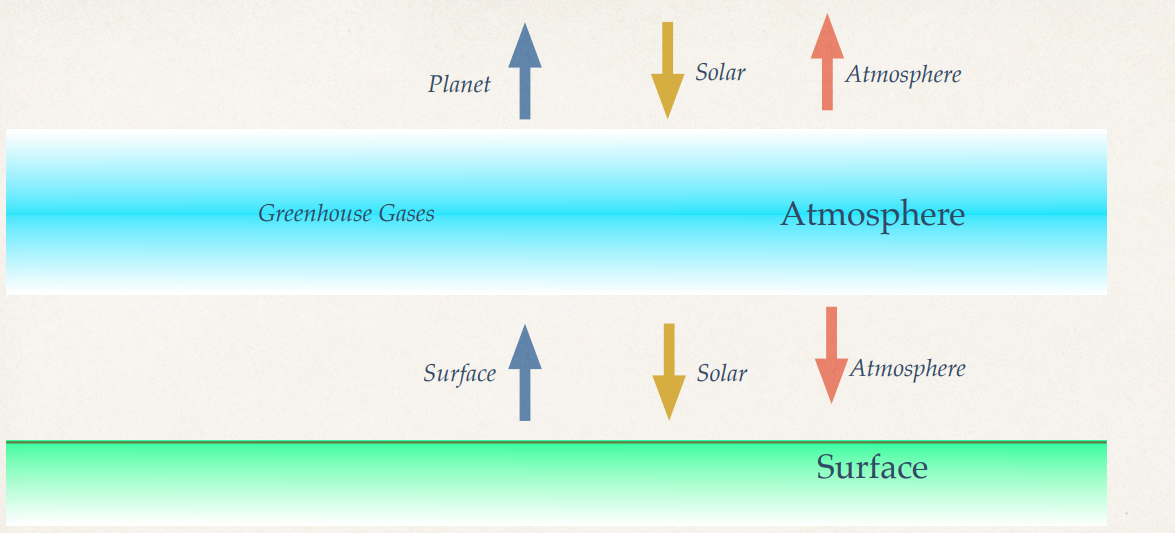
\includegraphics[width=0.5\linewidth]{uploads/Screenshot 2024-11-20 114831.png}
    \caption{Two-layer atmosphere}
    \label{fig:two layer}
\end{figure}
Lets’ look at different situations. 
\begin{enumerate}
    \item First assume the atmosphere does not absorb the solar radiation ($\epsilon = 1$): the atmosphere is totally transparent to solar radiation; and the transmissivity of the atmosphere is 0.0, no emission from the atmosphere:
$$F_S=\frac{S(1-\alpha)}{4}=238 \,\text{W/m}^2 \,\,\text{and}\,\, F_a=0$$
    that is the same balance as before when we didn't account for atmosphere
    \item Let’s allow now for some absorption of terrestrial radiation and the transmissivity of the atmosphere is 0.5:
    $$F_S= 396 \,\text{W/m}^2 \quad, F_a=158 \, \text{W/m}^2$$
    $$T_S= 289 \,\text{K}\approx 15°\text{C} \quad T_a=230 \, \text{K}\approx -43°\text{C}$$
    meaning that even with less than 0.5, the presence of atmosphere will give $T$ above 0°C. Opacity of the atmopshere is what makes possible the liquid water. 
    \item Assume a very opaque atmosphere the transmissivity is 1.0:
    $$F_S=476 \,\text{W/m}^2 \quad F_a=238 \, \text{W/m}^2$$
    $$T_S= 302 \,\text{K}\approx 28°\text{C} \quad T_a=254 \, \text{K}\approx -19°\text{C}$$
\end{enumerate}
\textcolor{RoyalBlue}{Opacity}: greenhouse work %CHECK.
\subsection{Three-layer atmosphere}
%If you are in continuous conditions the net flux between the fluxes up and down and the heating is proportional to the flux divergent that is the net balance between the 2 level is different
\begin{figure}[h!]
    \centering
    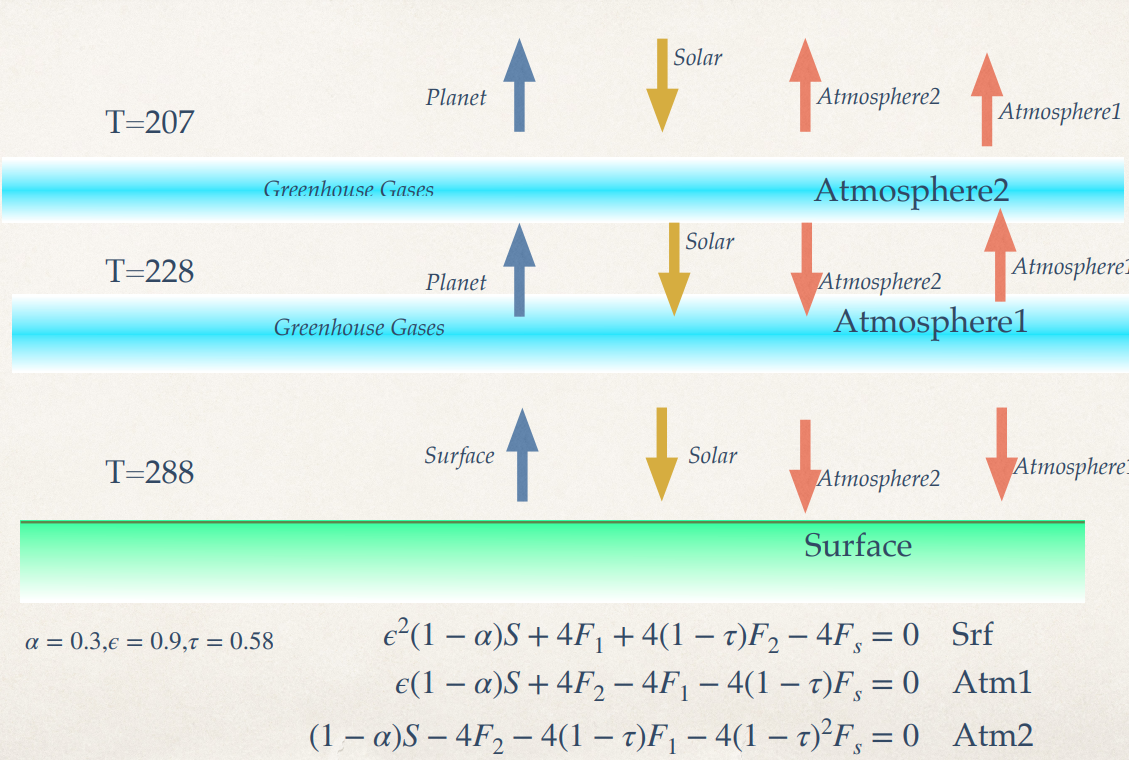
\includegraphics[width=0.65\linewidth]{uploads/Screenshot 2024-11-20 121339.png}
    \caption{Three-level atmosphere flux balance}
    \label{fig:three level}
\end{figure}
Remembering Kirchhoff’s law ( emissivity is equal to absorptivity), we
can introduce the temperature relations, we still consider the surface as a
black body $$F_S=\sigma T^4 \,\,\, F_1=\tau\sigma T_1^4 \,\,\, F_2=\tau\sigma T_2^4$$
\paragraph{Radiative equilibrium.} The transfer equation describes the behavior in the continuous case: 
$$\frac{dF^{\downarrow}}{d\tau}=B-F^{\downarrow} \qquad  \frac{dF^{\uparrow}}{d\tau}=F^{\uparrow}-B$$
where $B=\sigma T^4$ is the blackbody emission, $\tau$ the optical depth linked to the geometric height by $d\tau=-e_Ldz$. If we are in continuous conditions the net flux is $N=F^{\uparrow}-F^{\downarrow}$ and the long wave heating is proportional to the net flux divergence $-\frac{\partial N}{\partial z}$. SO, 
$$\frac{d}{d\tau}F^{\downarrow}e^{\tau}=Be^{\tau}\quad \frac{d}{d\tau}F^{\uparrow}e^{-\tau}=-Be^{-\tau}$$
At equilibrium there is no radiative heating, so:
$$\frac{\partial}{\partial z}(F^{\uparrow}-F^{\downarrow})=0\rightarrow\frac{\partial}{\partial\tau}(F^{\uparrow}-F^{\downarrow})$$
in general this is not satisfied because the air is in motion, but suppose that such equilibrium exist, then the incoming solar radiation is balanced by OLR, $F^{\uparrow}_T=F^{\uparrow}(\tau=0)=S$, so we get the boundary conditions at the top:
$$F^{\downarrow}=0 \quad F^{\uparrow}=F^{\uparrow}_T \quad \text{at} \, \, \tau=0$$
then the solution is 
$$F^{\downarrow}=\frac{\tau}{2}F^{\uparrow}_T \quad F^{\uparrow}=(1+1/\tau )F^{\uparrow}_T \quad B=\frac{(1+\tau)}{2}F^{\uparrow}_T $$
The contribute from each level OLR is:
$$OLR_S=(1-\tau)^2\sigma T^4_S \qquad OLR_1=\tau(1-\tau)\sigma T_1^4 \qquad OLR_2=\tau\sigma T_2^4$$
add perturbation (change a little bit the opacity)
$$OLR_S=(1-\tau-\Delta\tau)^2\sigma T^4_S \qquad OLR_1=(\tau+\Delta\tau)(1-\tau-\Delta\tau)\sigma T_1^4 \qquad OLR_2=(\tau+\Delta\tau)\sigma T_2^4$$
we'll get different curves with different temperature.
\begin{figure}[h!]
    \centering
    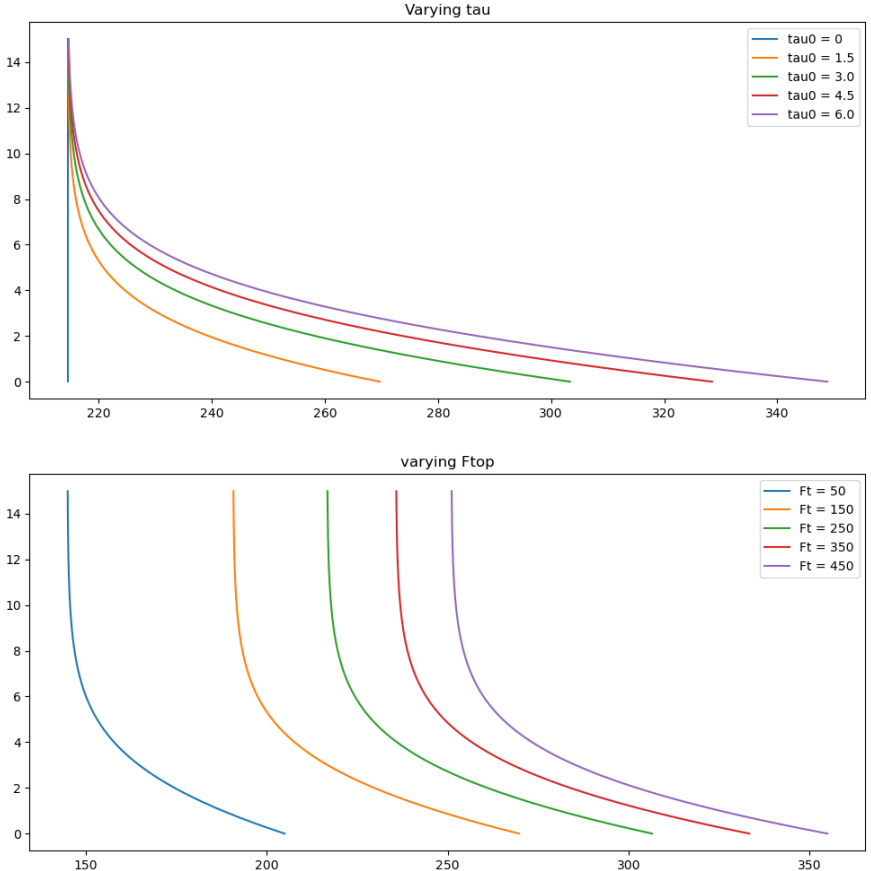
\includegraphics[width=0.5\linewidth]{uploads/Screenshot 2024-11-20 125556.png}
    \caption{The change in $OLR$}
    \label{fig:enter-label}
\end{figure}
Computing the change in $OLR$:
$$\Delta OLR_S\approx\Delta\tau[-2(1-\tau)]\sigma T_S^4 \qquad \Delta OLR_1\approx\Delta\tau(1-2\tau)\sigma T_1^4 \qquad \Delta OLR_2=\Delta\tau\sigma T_2^4$$
The factor that is the change of $OLR$ that corresponds to the change of opacity is called \textit{radiative forcing} and is 
\begin{equation}\label{eq.radiative forcing}
    R\approx-\Delta OLR
\end{equation}
\subsection{Many more layers}
Radiative equilibrium for 26 levels, with a realistic radiation calculation and observed components gases, with transmissivity and absorption coefficients ($T$ profile with vertical coordinate $p$).
\begin{figure}[h!]
    \centering
    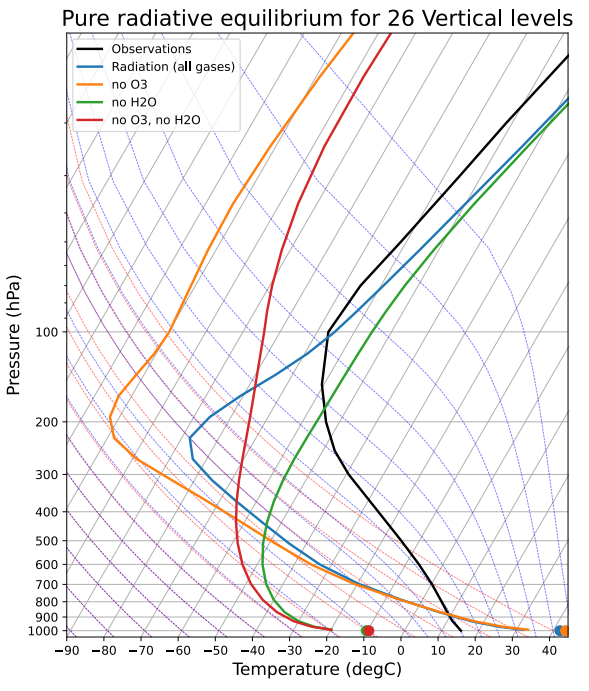
\includegraphics[width=0.5\linewidth]{uploads/Screenshot 2024-11-20 130113.png}
    \caption{the black line corresponds to the observations; the blue to the component of the atmosphere, it decreases with $T$ but in the stratosphere it changes inclination; the orange is without the ozone, responsable for the change of the slope in the stratosphere; the green one is without the water meaning that most of the opacity of the atmosphere disappears suddently, at the bottom $T$ is very cold; red without ozone and water, isotherm basically there is no atmosphere.}
    \label{fig:enter-label}
\end{figure}
The stratosphere is not still, we have convection: some of energy of the layer is brought up by radiation where it must be dispased?? by radiation So radiative equilibrium is possible but it must be modified. So these errors must be eliminated by radiation????? %martiii che cazz hai scritto dc
The most important thing of water vapor is cooling $\rightarrow$ radiative convective equilibrium. 



Two layers will be mixed until thanks to gravity light layers will sink below heavier layers.
\subsection{Convection}
\begin{figure}[h!]
    \centering
    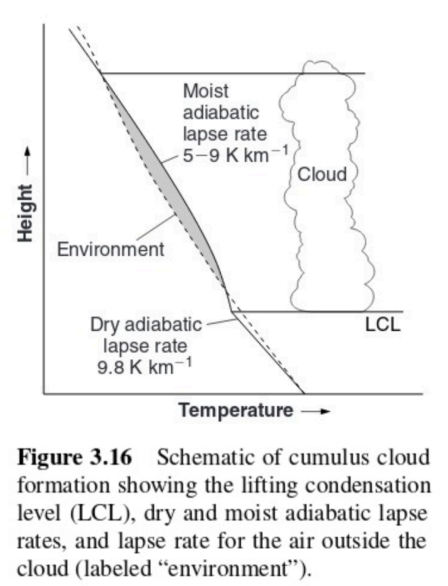
\includegraphics[width=0.5\linewidth]{uploads/Screenshot 2024-11-20 130640.png}
    \caption{}
    \label{fig:enter-label}
\end{figure}
\begin{figure}[h!]
    \centering
    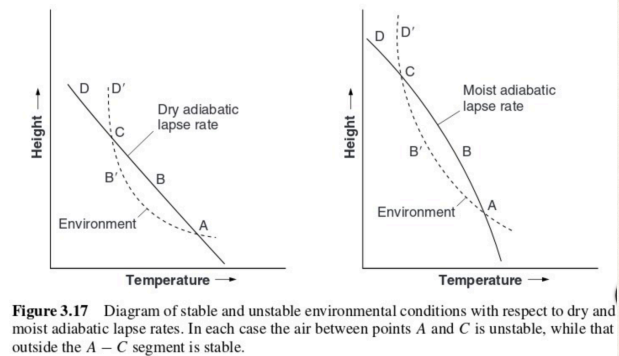
\includegraphics[width=0.5\linewidth]{uploads/Screenshot 2024-11-20 130727.png}
    \caption{}
    \label{fig:enter-label}
\end{figure}
Indicate with $T_r$, $q_r$ the equilibrium profile of temperature and moisture, then the convection must satisfy, if far from saturation (reference level), separately:
$$\int_{b_B}^{p_T}c_p(T_r-T_i)dp \qquad \int_{b_B}^{p_T}c_p(q_r-q_i)dp$$
where the integration goes from the bottom to the top of the convective layer. So you have the amount of extra energy that your system has with respect to the reference profile, you integrate over the entire level where you get divergence, if you have condensation, so you integrate where energy is condensed and profile is stable.
If precipitation occur, then the total enthalpy is conserved: 
$$\int_{b_B}^{p_T}c_p(h_r-h_i)dp \qquad h=c_pT+Lq$$
$T_r\rightarrow$ dry adiabat before saturation, moist adiabat after.
$q_r\rightarrow$ corresponding moisture. 
Identify the unstable profile, readjust  in such a way that reastablize??: upon conserved energy and you do with dry and then moist iterating the process. In this way I can include convection in my radiative equilibrium model: circulation in the column $\rightarrow$ check all radiative fluxes $\rightarrow$ take care about convection (convection adjustments).
\subsection{Radiative Convective Equilibrium}
Now I get this kind of thing, as I have movement I have to reach equilibrium (I can't solve an algebraic operation for equilibrium). The radiative convective equilibrium is similar to observations, especially for troposphere, the equilibrium in the troposphere is similar to the equilibrium between convection and radiation. The black line is the tendency, because it is not zero, it is not the equilibrium jet, I need it to be zero. The unbalance is mostly in the longwave, the short wave is sort of at equilibrium. Convection (contribution for the time tendency that is coming from convection) plays well in the lower levels: the first layer is unstable and the convective adjustment fixed it creating an adjustment in $T$. As I go forward, the convection goes up and the mixing ration stats to stabilize. We can see that there's almost balance in the lower level, the warm is coming from solar radiation and convection: take the heat net splitting it up and disposed by two other processes. Convection is not capable of getting really high. The energy balance in the troposphere is convection against all of the rest, so convection brings up as long-wave is emitting 
\begin{figure}[h!]
    \centering
    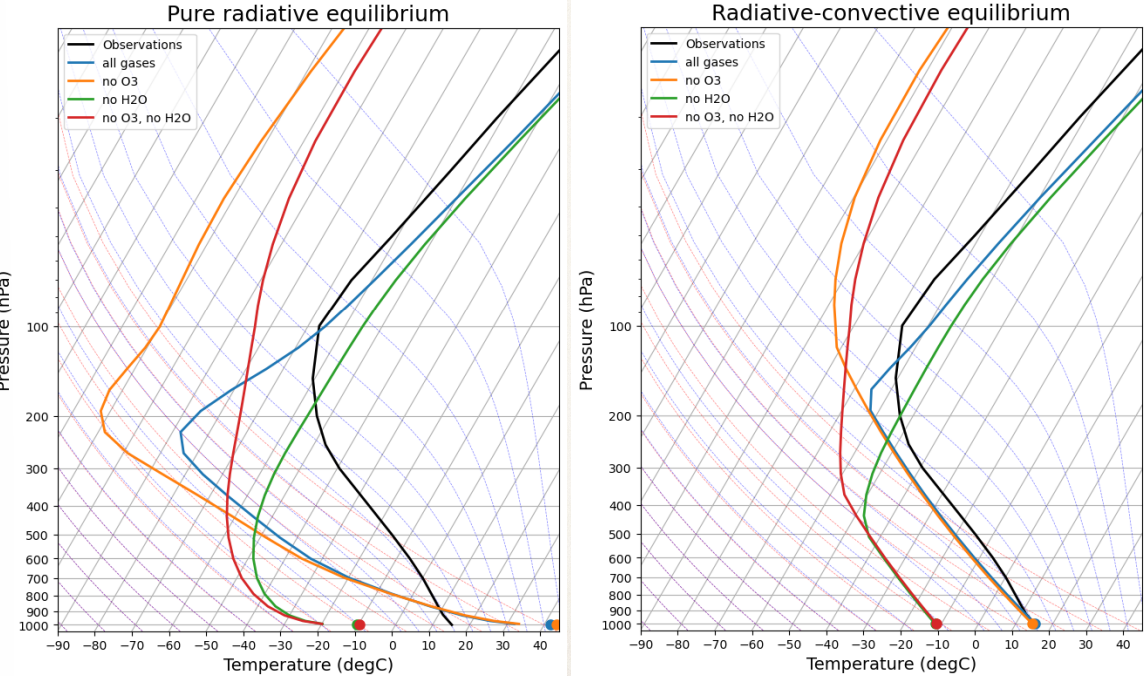
\includegraphics[width=0.5\linewidth]{uploads/Screenshot 2024-11-20 131319.png}
    \caption{Radiative Convective equilibrium}
    \label{fig:enter-label}
\end{figure}